\chapter{Sample a Test Set}
The test set will be used to evaluate performance of a very final model
and forecast the score in the competitions leaderboard. It may seems like
it's to early to create a test set, but I'll do it to prevent data snooping.

I'm going to do stratified sampling with scikit-learn's StraifiedShuffleSplit
to maintain equal ratio of men and women in the train set and the test set.
Women seem to have had a better chance of surviving due to the "women and
children first" protocol for loading lifeboats.

First, let's check how many passengers survived. There are 342 survived 
passengers and 549 drowned passengers in the dataset. Figure 
\ref{number_of_survivors} illustrates these numbers.

\begin{figure}[!ht]
	\centering
	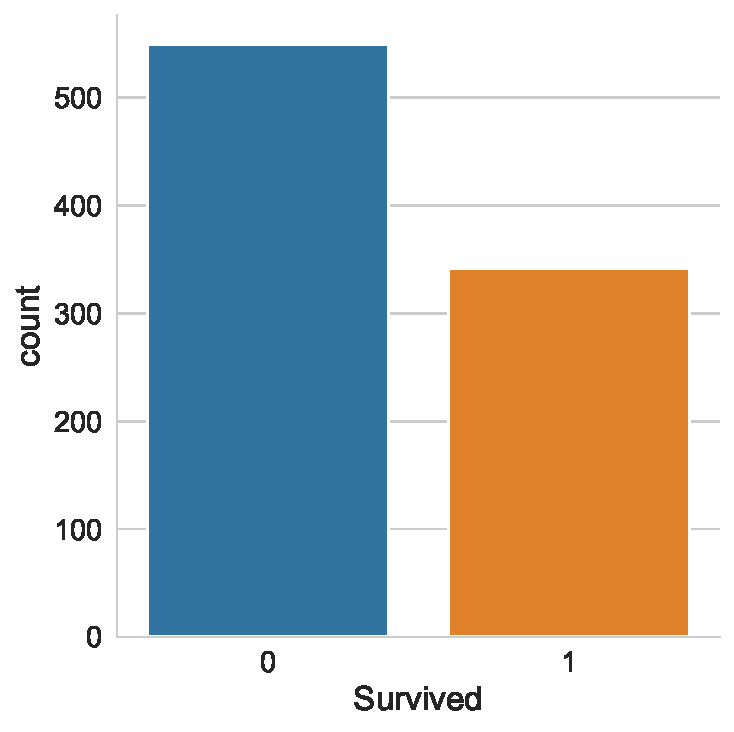
\includegraphics[width=0.5\textwidth]{number_of_survivors}
	\caption{Number of survived and drowned passangers in whole dataset.}
	\label{number_of_survivors}
\end{figure}

\begin{figure}[!ht]
	\centering
	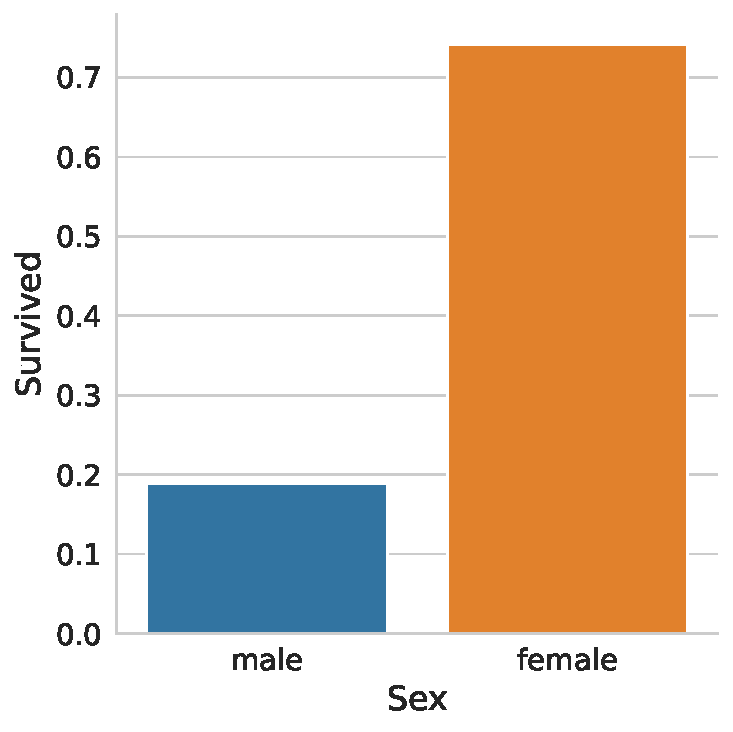
\includegraphics[width=0.5\textwidth]{proportion_of_survived_women}
	\caption{Proportions of survived men and women.}
	\label{proportion_of_survived_women}
\end{figure}

\begin{figure}[!ht]
	\centering
	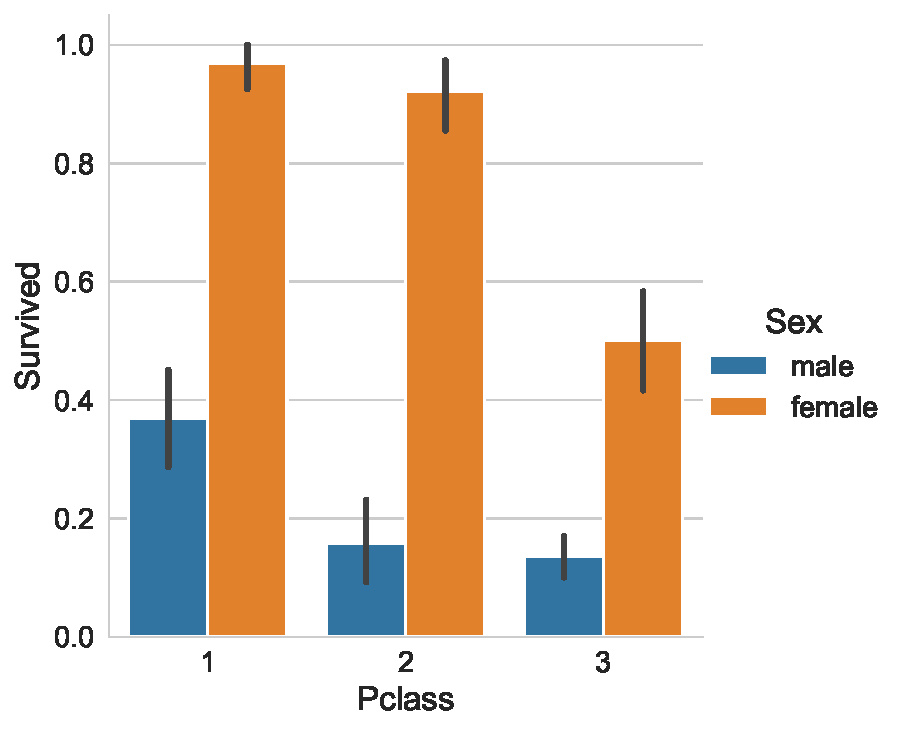
\includegraphics[width=0.5\textwidth]{proportion_of_survived_women_among_pclasses}
	\caption{Proporotion of survived women and men in each \textbf{"Pclass"}.}
	\label{proportion_of_survived_women_among_pclasses}
\end{figure}